\documentclass[12pt]{article}

\usepackage{amsmath,amsthm}
\usepackage{amsfonts}
\usepackage[psamsfonts]{amssymb}
\usepackage{palatino,euler}
\usepackage{graphicx}
\usepackage{hyperref}
\usepackage[french]{babel}
\usepackage{gensymb}
\usepackage{siunitx}
\usepackage[margin=1.25in]{geometry}
\usepackage{tikz}

\newcommand\critical{\SI{3.98}\celsius}
\numberwithin{figure}{section}
\numberwithin{table}{section}

\title{MAT1460\\[3ex]Fermeture de la patinoire naturelle du Lac aux Castors}
\author{Chen, Siying\\[1ex] Labont\'e, Pierre-Luc\\[1ex]Higgins, Philip\\[1ex] Grenier, David}
\date{}
\begin{document}

\maketitle
\thispagestyle{empty}
\vfill
\begin{center}
Universit\'e de Montr\'eal

\today
\end{center}
\clearpage

\tableofcontents
\clearpage
\section{Introduction}

Dans le cadre de travaux effectu\'es par la Ville de Montr\'eal au Lac aux Castors le probl\`eme de
polif\'eration d'algues a \'et\'e r\'egl\'e. Toutefois, la patinoire hivernale naturelle est
d\'esormais ferm\'ee en vertu d'un accident hivernale reli\'e \`a la qualit\'e de la glace. Les
citoyens ne pourront d\'esormais plus jouir de cette activit\'e au Lac aux Castors.

Le r\'echauffement plan\'etaire \'etant d\'esormais une r\'ealit\'e scientifiquement accept\'ee les
gestionnaires ont bl\^am\'e la situation sur des temp\'eratures plus \'elev\'ees qu'autrefois.
Toutefois, une cons\'equence directe des travaux est que la profondeur du lac a augment\'e de fa\c
con significative. Il est donc possible qu'il soit tout simplement plus difficile d'obtenir une
\'epaisseur de glace suffisante en raison du volume d'eau plus important \`a refroidir.

Nous avons donc construit certains mod\`eles permetant de v\'erifier l'impact des raisons
ci-haut mentionn\'es sur la qualit\'e de la glace.

\section{Impact de la temp\'erature}

Nous ne crayons pas \^etre en mesure de r\'epondre de fa\c con satisfaisante \`a la r\'ealit\'e du
r\'echauffement plan\'etaire. Nous pensons toutefois v\'erifier le bienfond\'e de l'argument de la
Ville de Montr\'eal sur la cause ultime de l'accident de l'hiver 2016-2017 qui est survenu apr\`es
les travaux de r\'efections.

Nous allons d'abord d\'eterminer si il y a une diff\'erence statistiquement significative dans les
temp\'eratures enregistr\'ees aux cours des ann\'ees r\'ecentes \`a celles historiques. Il est
entendu que la condition de la glace d\'epend des temp\'eratures ext\'erieures et nous allons donc
aussi tenter de mesurer le niveau de corr\'elation entre les temp\'eratures observ\'ees et les
donn\'ees d'ouverture des patinoires de l'\^Ile de Montr\'eal~\cite{PatHist}.

\subsection{Hypoth\`eses}

Nos hypoth\`eses sont principalement ax\'ees sur la nature des donn\'ees que nous avons disponibles:

\begin{enumerate}
    \item Nous supposons que les temp\'eratures ext\'erieures sur l'\^Ile de Montr\'eal sont
        uniform\'ement distribu\'ees;
    \item Lorsque les donn\'ees sont absentes en d\'ebut d\'ecembre et fin mars, nous supponsons que
        les patinoires sont ferm\'ees puisque hors-saison;
    \item Nous supposons les donn\'ees collectives sur les conditions des patinoires sont fiables;
    \item Nous assumons que l'\'ecart-type de temp\'erature donn\'ee par le minist\`ere est
        l'\'ecart-type r\'eel des temp\'eratures d'hivers avec lesquels nous comparons~\cite{AvgTemp};
    \item On suppose que s'il y a effectivement r\'echauffement plan\'etaire que ce dernier
        n'affecte pas significativement l'\'ecart-type.
\end{enumerate}

\subsection{Augmentation de la temp\'erature}

En utilisant les donn\'ees de temp\'eratures disponible~\cite{TempHist}, nous avons effectu\'e un
test de diff\'erence de moyennes pour d\'eterminer si les temp\'eratures moyennes des 10 derni\`eres
ann\'ees \'etaient semblable \`a celles des 30 derni\`eres ann\'ees~\cite{MeteoTemp}. La table
\ref{vars:hyptest} en donne les variables.

\begin{table}
    \centering
    \begin{tabular}{|l|l|r|}\hline
        Variable &Description &Valeur\\\hline
        $\mu_T$ &Moyenne de temp\'erature d\'ecembre-mars, 1981-2010 &-\SI{6.80}\celsius\\\hline
        $\sigma_T^2$, $\sigma_t^2$ &\'Ecart-type donn\'e par le minist\`ere &\SI{2.25}\celsius\\\hline
        $\mu_t$ &Moyenne \'echantillonnale d\'ecembre-mars &-\SI{5.06}\celsius\\\hline
        $n_T$ &Ann\'ees de temp\'eratures historique enregistr\'ees &30\\\hline
        $n_t$ &Ann\'ees de temp\'eratures r\'ecentes &10\\\hline
    \end{tabular}
    \caption{Test d'hypoth\`ese - \'echantillon 2008-2017}\label{vars:hyptest}
\end{table}

\begin{align*}
    H_0&: \mu_T - \mu_t = 0\\
    H_A&: \mu_T - \mu_t < 0\\
    p_\text{valeur} &= \frac{\mu_T - \mu_t}{\sqrt{\frac{\sigma_T^2}{n_T} + \frac{\sigma_t^2}{n_t}}} = \frac{\mu_T - \mu_t}{\sigma_T\sqrt{\frac1{n_T}+\frac1{n_t}}}\\
                    &= \frac{-6.8 + 5.06}{\sqrt{2.25}\sqrt{\frac1{30}+\frac1{10}}} = -3.17
\end{align*}

Notre statistique de test \'etant tr\`es faible nous \'ecartons l'hypoth\`ese que les temp\'eratures
r\'ecentes sont dans les normes hivernales. Nous ne pr\'etendons rien ici sur le r\'echauffement
plan\'etaire, mais seulement que les temp\'eratures des 10 derni\`eres ann\'ees sont
significativement plus \'elev\'ees.

\subsection{Corr\'elation des jours d'ouverture des patinoires}

Nous avons aussi extrait les donn\'ees d'ouverture des patinoires de l'\^Ile de Montr\'eal. Nous
avons concentr\'e nos efforts sur les donn\'ees des saisons 2008 \`a 2013, ann\'ees pour lesquels
nous avions les donn\'ees les plus robustes et ce pour les mois de D\'ecembre \`a Mars.

Nous avons \'etabli deux mesures (voir table \ref{data:predict}) pour v\'erifier la corr\'elation entre les temp\'eratures
observ\'ees et l'ouverture des patinoire. La premi\`ere est le nombre de jours o\`u
la temp\'erature maximale est au plus \SI0\celsius. La seconde est plus complexe, on
ne comptabilisera une journ\'ee que si les crit\`eres suivants sont satisfaits:

\begin{enumerate}
    \item La temp\'erature moyenne de la journ\'ee est au plus \SI0\celsius;
    \item Une surface n'est patinable que si la journ\'ee est indirectement pr\'ec\'ed\'ee de deux
        nuits cons\'ecutives de temp\'eratures minimales d'au plus -\SI{10}\celsius;
    \item Indirectement signifie que la journ\'ee n'est pas s\'epar\'ee des nuits froides par
        trois jours cons\'ecutifs de temp\'erature moyenne sup\'erieure \`a \SI0\celsius.
\end{enumerate}

\begin{table}
    \centering
    \begin{tabular}{|l|r|r|r|r|}\hline
        Ann\'ee &Temp moyenne &Pr\'ediction 1 &Pr\'ediction 2 &Ouvertures\\
                &(\si\celsius) & & &(nombre)\\\hline
        2017 &-4.92 &59 &82 &\\\hline
        2016 &-3.96 &52 &70 &\\\hline
        2015 &-6.69 &74 &89 &\\\hline
        2014 &-6.59 &72 &90 &\\\hline
        2013 &-5.05 &58 &61 &\\\hline
        2012 &-2.57 &50 &65 &57\\\hline
        2011 &-4.78 &66 &69 &56\\\hline
        2010 &-5.26 &65 &69 &55\\\hline
        2009 &-5.53 &72 &77 &62\\\hline
        2008 &-5.26 &61 &91 &62\\\hline
        Moyenne &-5.06 &62.0 &76.3 &58.4\\\hline
    \end{tabular}
    \caption{Pr\'edictions 1 \& 2 et jours d'ouverture r\'eel}\label{data:predict}
\end{table}

On voit en figure \ref{predictions} la droite des moindres carr\'es entre nos deux pr\'edictions et
les temp\'eratures moyennes saisonni\`eres. En particulier, la pr\'ediction 1 \`a une corr\'elation
forte n\'egative $R = -0.892$.

\begin{figure}
    \centering
    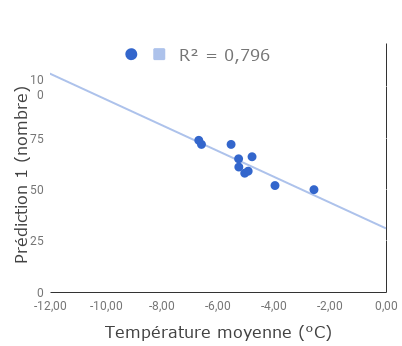
\includegraphics[scale=0.5]{Prediction1.png}
    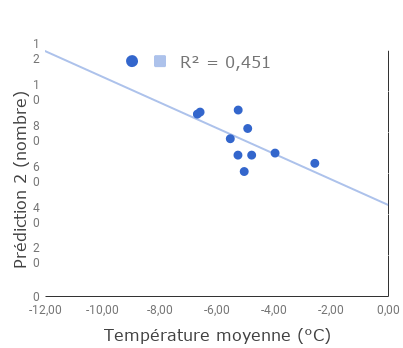
\includegraphics[scale=0.5]{Prediction2.png}
    \caption{Pr\'edictions 1 \& 2 contre les temp\'eratures moyennes saisonni\`eres}\label{predictions}
\end{figure}

Nos pr\'edicteurs \'etant reli\'es aux temp\'eratures moyennes saisonni\`eres, nous pensons que
s'ils sont efficaces pour pr\'edire les jours d'ouverture r\'eels, que nous aurons une bonne mesure
de l'impact des augmentations de temp\'eratures.

Le r\'esultat d'un test d'hypoth\`ese d'une diff\'erence de moyenne est indiqu\'e \`a l'\'equation
\eqref{test:days}. Notre \'echantillon \'etant petit nous avons effectu\'e un test de Student soumis
aux variables de la table \ref{vars:predict}. On voit qu'on ne peut donc pas \'ecarter la
possibilit\'e que notre $1^\text{er}$ pr\'edicteur est repr\'esentatif des jours d'ouverture r\'eel. 

\begin{table}
    \centering
    \begin{tabular}{|l|l|r|}\hline
        Variable &Description &Valeur\\\hline
        $n_1$, $n_2$ &Ann\'ees de donn\'ees de patinoires ouvertes &5\\\hline
        $s$ &Estimateur de la diff\'erence de moyenne &\\\hline
        $s_1$, $s_2$ &\'Ecart-type \'echantillonnal &\\\hline
        $\mu_1$ &Moyenne du pr\'edicteur 1 &\\\hline
        $\mu$ &Moyenne des jours d'ouverture &\\\hline
    \end{tabular}
    \caption{Variables pour les ann\'ees de donn\'ees pertinentes 2008-2012}\label{vars:predict}
\end{table}

\begin{align}
    H_0 &: \mu_1 - \mu = 0\notag\\
    H_A &: \mu_1 - \mu \ne 0\notag\\
    s &= \sqrt{\frac{(n_1-1)s_1^2 + (n_2-1)s_2^2}{n_1+n_2-2}} = \sqrt{39}\notag\\
    T_{\mu_1-\mu} &= \frac{\mu_1 - \mu}{s\sqrt{\frac1{n_1}+\frac1{n_2}}} = 1.114\label{test:days}
\end{align}

Sa droite des moindres carr\'es est donn\'ee par l'\'equation \eqref{eq:y}. Cette derni\'ere nous
dis que l'impact d'une augmentation de temp\'erature moyenne annuelle d'un \si{\celsius} se
traduirat par une perte de 6.72 jours de patinage par ann\'ee.

\begin{equation}
    y = -6.72x + 31.2\label{eq:y}
\end{equation}

Les mod\`eles actuels nous disent que la temp\'erature globale devrait augmenter de \SI4{\celsius}
d'ici 2100~\cite{GlobalRaise} relativement \`a la temp\'erature pr\'e-industrielle. Toutefois
l'impact Canadien d'une telle augmentation serait le double de l'impact global~\cite{CanadaRaise}.
Nous interpr\'etons cette derni\`ere comme une augmentation d'environ \SI6{\celsius} au cours des
prochains 80 ans et donc \si{0.75}{\celsius} par d\'ec\'enie.

\subsection{Validit\'e des r\'esultats}

Il n'est pas surprenant que notre premier pr\'edicteur soit fortement corr\'el\'e avec les moyennes
de temp\'erature annuelles. Quoique simple, ils donnent tous deux des valeurs raisonnable si bien
que nous n'avons pas cru bon d'effectuer une correction. Nous nous fions toutefois sur la
communaut\'e scientifique en ce qui attrait au r\'echauffement plan\'etaire. Cette derni\`ere
question \'etant beaucoup plus sophistiqu\'ee nous ne parlerons de l'impact sur la qualit\'e des
patinoires qu'en supposant leurs conclusions correcte.

\section{Impact de la profondeur}

Nous discuterons ici de l'effet de la profondeur du plan d'eau sur les conditions de glace. En
particulier, nous cherchons \`a savoir si l'excavation du lac~\cite{Lac} \`a contribu\'e de fa\c con
importante \`a la fermeture de la patinoire.

\subsection{Hypoth\`eses}

Afin de d\'eterminer l'impact de la profondeur sur la formation de la glace nous allons encadrer la
question des simplifications suivantes:

\begin{enumerate}
    \item Nous allons consid\'erer l'air ext\'erieur comme un puit de chaleur vaste dont la
        temp\'erature ne sera pas affect\'ee par la chaleur du lac;
    \item Similairement, nous allons traiter le sol comme une source de chaleur in\'epuisable;
    \item Nous n'allons \'evaluer que la perte d'\'energie du lac en terme de la conduction thermique
        et ignorer les contributions en radiation et \'evaporation~\cite{Evap};
    \item Nous supposons la temp\'erature ext\'erieure constante;
    \item Nous supposons aussi la temp\'erature du sol constante et uniform\'ement distribu\'ee;
    \item Nous ne connaissons pas les conductivit\'e thermiques en surface et au fond du lac, mais
        nous allons les consid\'erer respectivement identiques pour nos deux lacs;
    \item Nous ne connaissons pas la nature de l'interface en surface et au fond du lac pour le
        calcul de flux thermique et son \'epaisseur. Nous allons toutefois les consid\'erer
        identiques pour nos deux lacs.
\end{enumerate}

\subsubsection{Temp\'erature ext\'erieure constante}

Pour obtenir une r\'eponse r\'ealiste une simulation ou une utilisation judicieuse de probabilit\'es
nous permettrait d'inclure une fluctuation de temp\'erature. En particulier, nous savons que la
chaleur transmise entre deux corps est proportionnelle \`a la diff\'erence de temp\'erature entre
ces derniers~\cite{Fourier} et il serait pr\'eferable de ne pas n\'egliger cette composante.

Toutefois, ce m\'ecanisme est identique pour la chaleur d\'egag\'ee en surface et celle re\c cue par
le fond du lac. S'il y a une diff\'erence importante de variation de temp\'erature le lac plus
profond recevra d'avantage de chaleur du sol et il n'est pas clair que d'ajouter une temp\'erature
ext\'erieure variable va am\'eliorer le mod\`ele.

Puisque nous \'evaluerons la diminution de temp\'erature d'un lac par la chaleur d\'egag\'ee par le
plan d'eau \`a l'air environnant il s'ensuit que la temp\'erature chutera en surface. La capacit\'e
thermique~\cite{CapTherm} massique du sol est inf\'erieure a celle de l'eau, toutefois le volume de
la terre est de loin sup\'erieur \`a celle d'un lac. Il semble que la temp\'erature ne varie que de
\SI2{\celsius}~\cite{QuoraTemp} au cours d'une ann\'ee et de \SI{0.3}{\celsius} \`a tous les dix
m\^etre de profondeur. Nous accepterons donc une temp\'erature constante en hiver de
\SI{6}{\celsius}~\cite{GeoTemp}.

\subsection{La convection thermique}

Il est connu que la densit\'e de l'eau augmente avec une diminution de
temp\'erature~\cite{WaterDensity} atteignant son maximum \`a \critical{} ce qui introduit un
processus de convection thermique~\cite{ConvNat}.

\begin{figure}
    \centering
    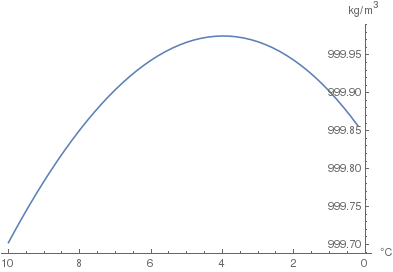
\includegraphics[scale=0.7]{WaterDensity.png}
    \caption{Densit\'e de l'eau}\label{water-density}
\end{figure}

Nous allons donc consid\'erer qu'un lac dont la temp\'erature est sup\'erieure \`a \critical, va
voir sa temp\'erature diminuer de fa\c con uniforme. D\'eterminer l'impact de la profondeur d'un
lac pour diminuer sa temp\'erature \`a \critical{} revient donc \`a mesurer le temps n\'ecessaire
pour obtenir les chaleurs respectives d\'egag\'ees.

\begin{figure}
    \centering
    \begin{tikzpicture}[scale=0.7]
        \shade[top color=blue!70,bottom color=brown] (0,3) -- (0,2) arc (180:360:3 and 0.5) -- (6,3)
        arc (0:180:3 and 0.5);
        \draw [<->] (3,3) -- (5.9,3) node [midway, above, scale=0.7] {$r$};
        \draw [<->] (6.3,3) -- (6.3,2) node [midway, right, scale=0.7] {$p_1$};
        \draw (3,3) ellipse (3 and 0.5);
        \draw (0,3) -- (0,2);
        \draw (6,3) -- (6,2);
        \draw [dashed] (0,2) arc (180:0:3 and 0.5);
        \draw (0,2) arc (180:360:3 and 0.5);
        \draw[line width=0.5mm, ->] (1.8,2.7) arc (95:445:1cm and 0.45cm);
        \draw[line width=0.5mm, ->] (4.2,2.7) arc (85:-260:1cm and 0.45cm);

        \shade[top color=blue!70,bottom color=brown] (7,3) -- (7,-1) arc (180:360:3 and 0.5) -- (13,3)
        arc (0:180:3 and 0.5);
        \draw [<->] (10,3) -- (12.9,3) node [midway, above, scale=0.7] {$r$};
        \draw [<->] (13.3,3) -- (13.3,-1) node [midway, right, scale=0.7] {$p_2$};
        \draw (10,3) ellipse (3 and 0.5);
        \draw (7,3) -- (7,-1);
        \draw (13,3) -- (13,-1);
        \draw [dashed] (7,2) arc (180:360:3 and 0.5);
        \draw [dashed] (7,-1) arc (180:0:3 and 0.5);
        \draw (7,-1) arc (180:360:3 and 0.5);
        \draw[line width=0.5mm, ->] (8.8,2.7) arc (95:445:1cm and 2cm);
        \draw[line width=0.5mm, ->] (11.2,2.7) arc (85:-260:1cm and 2cm);
    \end{tikzpicture}
    \caption{Convection \`a plus de \critical}\label{water-convection}
\end{figure}

\subsection{La conduction thermique (ou diffusion)}

Le sol \'etant un solide il n'est pas sujet \`a la convection tel l'eau du lac. Nous aurions une
meilleure approximation en consid\'erant le processus de diffusion qui, \`a un \'etat eventuel
stable, conduirait \`a une temp\'erature du sol lin\'eairement distribu\'ee~\cite{TempLinear}.
Toutefois, ces calculs seraient compliqu\'es et nous pensons pouvoir d\'eduire, par le th\'eor\`eme
de la moyenne~\cite{AvgValue}, qu'il existe une temp\'erature constante pour laquelle la
contribution en chaleur du sol sera la m\^eme que pour une temp\'erature distribu\'ee de fa\c con
plus r\'ealiste.

Remarquons aussi qu'en dessous de \critical, la densit\'e de l'eau se met \`a diminuer avec une
diminution de temp\'erature. Le processus de convection devient alors stable~\cite{HydroStab} et la
temp\'erature ne varie plus de fa\c con uniforme. On penses que la temp\'erature variera \`a
l'int\'erieur du corps tel la diffusion de la chaleur dans une tige, la profondeur aura donc quand
m\^eme un impact. Toutefois, il n'est plus n\'ecessaire \`a cette \'etape de refroidir le lac dans
son ensemble pour obtenir une formation de glace \`a la surface. Le refroidissement du lac doit donc
\^etre trait\'e diff\'eremment apr\`es l'atteinte de la temp\'erature uniforme de \critical.

\subsection{Au dessus de \SI4\celsius}

Nous allons tenter de d\'eterminer l'\'evolution, au dessus de \SI4{\celsius}, de la temp\'erature
de deux lacs id\'ealis\'es de profondeurs diff\'erentes. Nous appelerons ci-apr\`es les lac 1 et 2
comme \'etant le lac de r\'ef\'erence et le lac excav\'e sujettes aux variables suivantes:

\begin{table}
    \centering
    \begin{tabular}{|l|l|l|}\hline
        Variable &Description &Unit\'e\\\hline
        $Q$ &Chaleur &\si\joule\ (\si{\kilogram.\square\meter\per{\square\second}})\\\hline
        $T$ &Temp\'erature &\si{\kelvin}\\\hline
        $c_p$ &Capacit\'e thermique massique &\si{\joule\per{\kelvin\,\kilogram}}\\\hline
        $m$ &Masse &\si\kg\\\hline
        $C$ &Capacit\'e thermique &\si{\joule\per\kelvin}\\\hline
        $K$ &Conductivit\'e thermique &\si{\joule\per{\meter\,\second\,\kelvin}}\\\hline
        $\rho$ &Densit\'e de la substance &\si{\kilogram\per{\square\meter}}\\\hline
        $V$ &Volume &\si{\cubic\meter}\\\hline
        $r$ &Rayon d'un lac cylindrique &\si\meter\\\hline
        $A$ &Superficie &\si{\square\meter}\\\hline
        $p$ &Profondeur d'un lac cylindrique &\si\meter\\\hline
        $t$ &Temps &\si\second\\\hline
    \end{tabular}
    \caption{Variables}
\end{table}

Lorsqu'un corps subit une variation de temp\'erature l'energie transf\'er\'ee
(chaleur)~\cite{Q-equation} nous est donn\'ee par l'\'equation \eqref{eq:heat}.

\begin{align}
    Q &= C\Delta T\label{eq:heat}\\
    &= c_pm\Delta T\notag\\
    &= c_p\rho V\Delta T\notag\\
    &= c_p\rho (p\pi r^2p)\Delta T &&\text{(pour un lac cylindrique)}\notag
\end{align}

La capacit\'e thermique d'un corps $(C)$ est une propri\'et\'e extensive~\cite{Extensive} sa valeur
est directement proportionnelle \`a la masse du syst\`eme. Si la masse du second lac est le triple
du premier, il devra perdre trois fois plus d'\'energie pour atteindre la m\^eme temp\'erature.

La figure \ref{water-convection} nous montre un second lac expos\'e \`a la m\^eme surface
ext\'erieure. Sa superficie en contact avec le sol que est toutefois un peu plus importante. Nous
allons d'abord \'evaluer la chaleur \`a perdre pour atteindre \critical{} et ensuite le temps requis
pour perdre cette chaleur.

Les donn\'ees officielles sur la superficie et la profondeur du Lac aux Castors semblent difficile
\`a obtenir. Nous avons toutefois r\'eussi \`a estimer la superficie du lac \`a environ
\SI{18500}{\square\meter} (voir figure \ref{google-castor}). On nous informe aussi qu'en vertu des
travaux le lac est pass\'e d'une profondeur d'environ 2 \`a 7 m\^etres~\cite{Lac-Castor}.

\begin{figure}
    \centering
    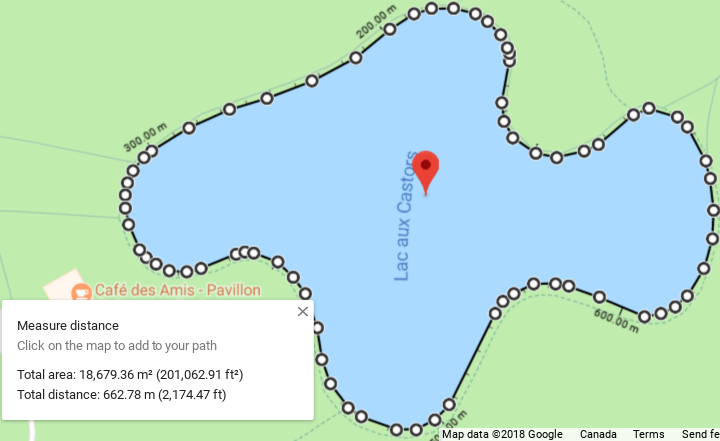
\includegraphics[scale=0.5]{Superficie.png}
    \caption{Superficie du Lac aux Castors}\label{google-castor}
\end{figure}

En ramenant ces donn\'ees \`a un lac cylindrique de superficie et volumes respectifs on obtient
les param\`etres ci-dessous pour effectuer nos calculs:

\begin{table}
    \centering
    \begin{tabular}{|l|l|r|}\hline
        Param\`etre &Description &Valeur\\\hline
        $c_p$ &Capacit\'e thermique massique de l'eau &\SI{4185.5}{\joule\per{\kelvin\,\kilogram}}\\\hline
        $T_\text{sol}$ &Temp\'erature du sol &\SI{279.15}\kelvin\ (\SI6\celsius)\\\hline
        $T_\text{air}$ &Temp\'erature de l'air &\SI{261.15}\kelvin\ (\SI{-12}\celsius)\\\hline
        $T_\text{init}$ &Temp\'erature initiale de l'eau &\SI{285.15}\kelvin\ (\SI8\celsius)\\\hline
        $T_\text{cible}$ &Temp\'erature \`a hydrostabilit\'e &\SI{277.13}\kelvin\\\hline
        $A_{lac}$ &Superficie du lac &\SI{18500}{\square\meter}\\\hline
        $p_1,p_2$ &Profondeur du lac et lac excav\'e &\SI2\meter, \SI7\meter\\\hline
        $\rho$ &Densit\'e de l'eau &\SI1{\kilogram\per{\cubic\meter}}\\\hline
        $K$ &Conductivit\'e thermique de surface &inconnue\\\hline
        $x$ &\'Epaisseur de l'interface de surface &inconnue\\\hline
        $\alpha$ &Ratio des constantes du fond contre surface &param\`etre\\\hline
    \end{tabular}
    \caption{Param\`etres}
\end{table}

On trouves les pertes de chaleur n\'ecessaire de nos deux lacs:

\begin{align*}
    r &= \sqrt{\frac{18500}\pi} = \SI{76.738}\meter\\
    C_1 &= c_pm_1 = c_p\rho p_1\pi r^2 = \num{1.549e8}\si{\joule\per\kelvin}\\
    C_2 &= c_pm_2 = c_p\rho p_2\pi r^2 = \num{5.420e8}\si{\joule\per\kelvin}\\
    \Delta T &= T_\text{cible} - T_\text{init} = \SI{-4.02}\kelvin\\
    Q_1 &= C_1\Delta T = -\num{6.226e8}\si\joule\\
    Q_2 &= C_2\Delta T = -\num{2.179e9}\si\joule
\end{align*}

On doit maintenant \'evaluer la chaleur \'emise par la surface et re\c cue par le fond du lac.
L'\'equation du flux thermique \eqref{eq:flux} n'est normalement pas applicable
directement~\cite{HeatFlow} puisqu'elle est typiquement utilis\'ee entre deux syst\`emes de masse et
capacit\'e thermique massique identiques. Aussi, la structure des interfaces entre a surface de
l'eau et l'air ambiant ainsi que celle du fond du lac nous sont inconnues. Nous ne pensons pas
pouvoir trouver la conductivit\'e thermique appropri\'ee ainsi que le gradient de temp\'erature
r\'eel.

\begin{align}
    \frac{\Delta Q}{\Delta t} = -KA\frac{\Delta T}x \label{eq:flux}
\end{align}

Nous allons donc absorber ces constantes dans la variable d'int\'egration. Pour simplifier les
calculs nous allons aussi absorber l'aire de la surface et exprimer les constantes pour le fond du
lac comme le produit d'un nouveau param\`etre qu'on fera varier. Nous n'obtiendront donc pas une
unit\'e de temps r\'eelle mais nous allons toutefois \^etre en mesure d'\'evaluer la diff\'erence
relative entre nos deux syst\`emes.

\begin{align}
    A_1 &= 2\pi r p_1 + \pi r^2 = \num{1.946e4}\si{\square\meter}\notag\\
    \frac{dQ_1}{dt} &=
        -KA_\text{lac}\frac{T_1(t) - T_\text{air}}x -\alpha KA_1\frac{T_\text{fond}-T_1(t)}x\notag\\
    &= \underbrace{KA_\text{lac}\frac{T_\text{air}-T_1(t)}x\
        -\alpha KA_1\frac{T_\text{fond}-T_1(t)}x}_{\tau = A_\text{lac}\frac Kxt}\notag\\
    \frac{dQ_1}{d\tau} &= T_\text{air} - T_1(\tau) - \alpha (T_\text{fond} -
        T_1(\tau))\label{eq:diff}\\
    \text{o\`u } T_1(\tau) &= T_\text{cible} - \frac{Q_1(\tau)}{C_1} \label{eq:temp}&&\text{(par l'\'equation \eqref{eq:heat})}
\end{align}

En substituant \eqref{eq:temp} dans l'\'equation \eqref{eq:diff} on obtient une \'equation
diff\'erentielle \`a variable s\'eparable qui n'est pas si difficile \`a r\'esoudre. En donnant les
conditions initiales ($Q(0) = 0$) on trouves $Q_1(\tau)$ et $Q_2(\tau)$. Apr\`es substitution dans
\eqref{eq:temp} on obtient les \'equations nous donnant l'\'evolution de la temp\'erature en fonction
de notre temps $\tau$.

\begin{align*}
    T_1(\tau) &=
        T_\text{init} +
            \left(1-e^{\textstyle -t\frac{\alpha A_1-A_\text{lac}}{C_1}}\right)
            \frac
                {A_\text{lac} T_\text{air} + (\alpha A_1-A_\text{lac})T_\text{cible} - \alpha A_1 T_\text{fond}}
                {\alpha A_1-A_\text{lac}}\\
    T_2(\tau) &=
        T_\text{init} +
            \left(1-e^{\textstyle -t\frac{\alpha A_2-A_\text{lac}}{C_2}}\right)
            \frac
                {A_\text{lac} T_\text{air} + (\alpha A_2-A_\text{lac})T_\text{cible} - \alpha A_2 T_\text{fond}}
                {\alpha A_2-A_\text{lac}}\\
\end{align*}

Ces derni\`eres \'etant inversibles, on a pu trouver le temps $\tau$ pour atteindre la perte de
chaleur recherch\'ee pour diverses valeurs de $\alpha$. On trace ainsi les courbes des chutes de
temp\'eratures pour les deux lacs.

\begin{figure}
    \centering
    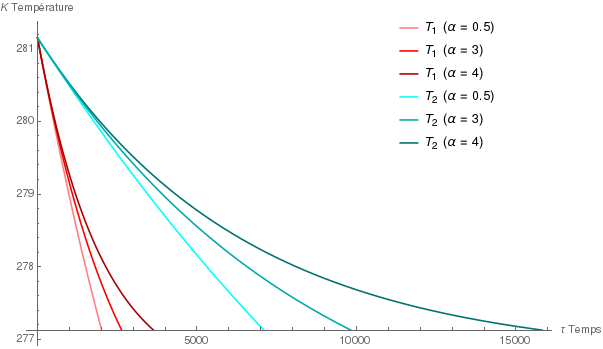
\includegraphics[scale=0.7]{Alpha.png}
    \caption{Chutes de temp\'eratures pour $\alpha \in \{0.5, 3, 4\}$.}
\end{figure}

\subsection{De \SI4{\celsius} \`a \SI0\celsius}

\subsection{Validit\'e des r\'esultats}

\section{Analyse}
\subsection{Discussion des r\'esultats}
\subsection{Forces et faiblesses}

\section{Conclusion}

\clearpage
\section{Bibliographie}
\begin{thebibliography}{Xyz}
    \bibitem{TempHist} \href{https://www.meteomedia.com/ca/api/sitewrapper/index?b=%2Fstatistics%2F&p=%2Fprevisions%2Fstatistiques%2Findex&url=%2Fstatistics%2Fcaqc0363%2Fmontreal%2F%2F%2F%3F}
        {M\'et\'eoM\'edia - Montr\'eal}
    \bibitem{PatHist} \href{http://donnees.ville.montreal.qc.ca/dataset/patinoires-historique}
        {Patinoire - historique des conditions}
    \bibitem{AvgTemp} \href{http://www.mddelcc.gouv.qc.ca/climat/surveillance/classification.htm}
        {Classification climatologique des temp\'eratures}
    \bibitem{MeteoTemp} \href{https://www.meteomedia.com/ca/api/sitewrapper/index?b=%2Fstatistics%2F&p=%2Fprevisions%2Fstatistiques%2Findex&url=%2Fstatistics%2Fcaqc0363%2Fmontreal%2F%2F%2F%3F}
        {Statistiques: Montr\'eal, Que\'ebec - M\'et\'eoM\'edia}
    \bibitem{GlobalRaise} \href{https://www.independent.co.uk/environment/global-warming-temperature-rise-climate-change-end-century-science-a8095591.html}
        {Worst-case global warming predictions}
    \bibitem{CanadaRaise} \href{https://www.canada.ca/fr/environnement-changement-climatique/services/changements-climatiques/science.html}
        {Science des changements climatiques}
    \bibitem{Lac} \href{https://www.ledevoir.com/politique/montreal/517828/patinoire-du-lac-aux-castors}
        {Montr\'eal abandonne la patinoire naturelle du lac aux Castors}
    \bibitem{Evap} \href{https://www.quora.com/How-does-evaporation-take-place-at-all-temperatures-whereas-boiling-takes-place-at-a-fixed-temperature-under-a-given-pressure}
        {How does evaporation take place at all temperatures}
    \bibitem{Fourier} \href{https://fr.wikipedia.org/wiki/Conduction_thermique#Loi_de_Fourier}
        {Loi de Fourier}
    \bibitem{CapTherm} \href{https://fr.wikipedia.org/wiki/Capacit%C3%A9_thermique_massique}
        {Capacit\'e thermique massique}
    \bibitem{WaterDensity} \href{http://www.open.edu/openlearn/science-maths-technology/the-oceans/content-section-3.2}
        {The density of fresh water and seawater}
    \bibitem{ConvNat} \href{https://fr.wikipedia.org/wiki/Convection_thermique#Convection_naturelle}
        {Convection naturelle}
    \bibitem{TempLinear} \href{https://fr.wikipedia.org/wiki/Conduction_thermique#Surfaces_planes_en_série}
        {Conduction Thermique - Profil des temp\'eratures}
    \bibitem{AvgValue} \href{https://fr.wikipedia.org/wiki/Th%C3%A9or%C3%A8me_de_la_moyenne}
        {Th\'eor\`eme de la moyenne}
    \bibitem{HydroStab} \href{https://fr.wikipedia.org/wiki/Gradient_thermique_adiabatique#Atmosph.C3.A8re_stable}
        {Stabilit\'e hydrostatique}
    \bibitem{Q-equation} \href{https://simple.wikipedia.org/wiki/Specific_heat#Usage}
        {Calculating heat}
    \bibitem{Extensive} \href{https://fr.wikipedia.org/wiki/Extensivit%C3%A9_et_intensivit%C3%A9_(physique)}
        {Extensivit\'e}
    \bibitem{Lac-Castor} \href{https://fr.wikipedia.org/wiki/Lac_aux_Castors_(Montr%C3%A9al)}
        {Lac aux Castors}
    \bibitem{SpecHeat} \href{https://www.engineeringtoolbox.com/specific-heat-capacity-d_391.html}
        {Specific heat of common Substances}
    \bibitem{NewtonLaw} \href{https://en.wikipedia.org/wiki/Newton%27s_law_of_cooling}
        {Newton Law of cooling}
    \bibitem{HeatFlow} \href{https://en.wikipedia.org/wiki/Rate_of_heat_flow}
        {Rate of heat flow}
    \bibitem{Conductivity} \href{https://www.engineeringtoolbox.com/thermal-conductivity-d_429.html}
        {Thermal Conductivity of common Materials and Gases}
    \bibitem{QuoraTemp} \href{https://fr.quora.com/Quelle-est-la-temp%C3%A9rature-de-la-terre-%C3%A0-10m-et-et-20m}
        {Quelle est la temp\'erature de la terre}
    \bibitem{GeoTemp} \href{http://www.sblais.com/default.asp?idpage=2377&idpageparent=2315}
        {La g\'eothermie}
\end{thebibliography}

\end{document}
